%==============================================================
% ICECE submission -- IEEE conference, A4, anonymous, 6-page target.
% (Submitted to ICECE. A different paper went to ICCIT 2026 -- these are
%  separate works, so there is no parallel submission.)
%
% ALL SIX FIGURES ARE KEPT. Only text was cut:
%   * CCS Concepts block (ACM-only, no IEEE equivalent)
%   * "Key Observations" and "Addressing the Research Problems"
%     -- both restated results given earlier
%   * "Final Configuration Evaluation" -- folded into one sentence in IV-A
%   * "Why Visual Features Dominate" -- its argument moved into IV-A
%   * bullet lists in I-A and II -- compressed to prose
%   * the CISF-mechanism paragraph in the discussion
%   * the separate baseline table, folded into Table I as two rows
%     (a table, not a figure -- its bar chart, Fig. 6, is still here)
%   * roughly a dozen paragraphs tightened without losing a claim
% The rest of the page was found by narrowing Fig. 1 to 0.80 textwidth, setting
% the tables footnotesize, and putting the column figures at 0.95 columnwidth.
% Every reviewer fix is retained: near-duplicate screening, validation-only
% threshold selection, the sealed single scoring, the retraction, the fusion
% verdict, per-class metrics and confidence intervals.
%
% NUMBERS. All regenerated from the deduplicated, group-aware runs:
%   duplicate_clusters.csv, adversarialgen_val148_sweep.csv,
%   adversarialgen_leakfree_clean_results.csv, ablation_grouped_summary.csv,
%   baselines_grouped_summary.csv, fusion_vs_cliponly.csv
%
% FIGURES required (figures/ or beside the .tex) -- all six, in this order:
%   Fig. 1  fig1_system_architecture.png          Sec. III-A, spans both columns
%   Fig. 2  fig2_modality_ablation.png            Sec. IV-A
%   Fig. 3  fig3_validation_threshold_sweep.png   Sec. IV-C
%   Fig. 4  fig4_shift_performance.png            Sec. IV-C
%   Fig. 5  fig5_confusion_matrices.png           Sec. IV-C
%   Fig. 6  fig6_baseline_comparison.png          Sec. IV-D
%
% REFERENCES: every arXiv-backed entry was checked against the arXiv record
% and RAGAR against the ACL Anthology. Still unverified, because no
% machine-readable record was consulted: multibanfake (IJIMDS 2025) and
% claaf (PLOS ONE 2025).
%
% DATASET FACTS verified against the distributed files, not assumed:
%   AdversarialGen is BALANCED (1,000 authentic + 1,000 manipulated), not
%   2,000 AI-generated images; every CSV carries article_id / source_dataset /
%   category, so provenance IS published. Article-level overlap is MEASURED,
%   not removed: 20 of the 194 sealed test images share an article with
%   training data, and excluding them moves accuracy by +0.7 to +1.1 points.
%   The screening claim in Sec. III-B is limited to image duplicates.
%
% BanFakeMM reference completed from the DataCite record for
% doi:10.17632/3r9s7wfbh5.1 (creators, year, version, publisher).
% No BLOCKING reference TODOs remain.
%==============================================================
\documentclass[conference,a4paper]{IEEEtran}
\IEEEoverridecommandlockouts

\usepackage{cite}
\usepackage{amsmath,amssymb,amsfonts}
\usepackage{graphicx}
\usepackage{booktabs}
\usepackage{multirow}
\usepackage{textcomp}
\usepackage{url}
\usepackage[section]{placeins}

% Keep floats near the text that discusses them rather than at the end.
\renewcommand{\topfraction}{0.92}
\renewcommand{\bottomfraction}{0.75}
\renewcommand{\textfraction}{0.06}
\renewcommand{\floatpagefraction}{0.65}
\renewcommand{\dbltopfraction}{0.92}
\setcounter{topnumber}{3}
\setcounter{bottomnumber}{2}
\setcounter{totalnumber}{4}

\graphicspath{{figures/}{./}}

\newif\ifblindsubmission
\blindsubmissiontrue      % conference requires anonymous submission

\newif\ifdraftnotes
\draftnotesfalse          % submission build: internal notes hidden

\newcommand{\sysname}{SignalCheck}

\begin{document}

\title{\sysname: Multimodal Bangla Fake News Image Detection --
Modality Ablation and Duplicate-Screened Distribution-Shift Evaluation}

\ifblindsubmission
  % Blind build: no author line at all. If the submission system assigns a
  % paper ID and asks for it on the manuscript, put it back here.
  \author{}
\else
  \author{\IEEEauthorblockN{1\textsuperscript{st} Given Name Surname}
  \IEEEauthorblockA{\textit{dept. name of organization} \\
  \textit{name of organization}\\ City, Country \\ email or ORCID}
  \and
  \IEEEauthorblockN{2\textsuperscript{nd} Given Name Surname}
  \IEEEauthorblockA{\textit{dept. name of organization} \\
  \textit{name of organization}\\ City, Country \\ email or ORCID}
  \and
  \IEEEauthorblockN{3\textsuperscript{rd} Given Name Surname}
  \IEEEauthorblockA{\textit{dept. name of organization} \\
  \textit{name of organization}\\ City, Country \\ email or ORCID}}
\fi

\maketitle

\begin{abstract}
Fake news detection for low-resource languages such as Bangla is held back by
the scarcity of image-centric training data and by evaluation protocols that
leak. This paper presents \sysname, a classifier for manipulated news imagery
circulating on Bangladeshi social media, built by ablating a multimodal
pipeline down to what the evidence supports. On the BanFakeMM benchmark, under
duplicate-aware grouped cross-validation, CLIP visual features dominate at
95.38 percent alone and no text-inclusive configuration differs beyond
fold-to-fold variation; OCR, near chance at 57.35 percent, is removed, and a
calibration analysis finds the caption-fusion pathway unjustified, so CLIP-only
is the configuration we recommend. Every
partition is screened for near-duplicates, the decision threshold is chosen on
a disjoint validation partition, and a sealed test partition is scored exactly
once. Zero-shot transfer to an unseen manipulation style costs 10.3 points of
accuracy and 21.2 points of fake-recall (95.38 to 85.1 percent; 96.15 to
75.0 percent); a validation-selected threshold recovers most of that without
retraining, reaching 91.2 percent and 96.0 percent. Supervised adaptation on
300 target-style images adds nothing measurable ($-1.5$ points, 95 percent CI
$[-4.6, +1.5]$); an earlier draft reported a gain here, which we retract.
\end{abstract}

\begin{IEEEkeywords}
Bangla fake news detection, multimodal misinformation, CLIP, XGBoost,
distribution shift, threshold calibration, near-duplicate leakage,
low-resource language processing
\end{IEEEkeywords}

%==============================================================
\section{Introduction}
%==============================================================

Bangladesh's social media ecosystem has become a primary vector for
manipulated news imagery, from digitally altered photocards and forged
documents to AI-generated video frames misattributed to public figures. Unlike
text-only misinformation, this content exploits the visual and textual channels
jointly: a viral image is judged not on its pixels alone but on the claim
attached to it as it spreads.

The problem is compounded by linguistic specificity. Most fake-news detection
methods are built on English datasets from Western platforms and presuppose
signals---dense comment threads, public retweet graphs---that are sparse or
structured differently in Bangladesh. Two further gaps follow. No large-scale,
organically collected corpus of manipulated Bangladeshi news images exists, so
training must rely on synthetic benchmarks. And same-distribution accuracy is
routinely reported as if it were real-world reliability, without a disjoint
evaluation---or, where one is reported, with the operating threshold tuned on
the very set used to report it.

This paper contributes a per-modality ablation that determines which
modalities earn their place, removing OCR and then the caption pathway; a
distribution-shift protocol with three named safeguards---near-duplicate
screening of every partition on image content, with residual article-level
overlap measured rather than assumed away; threshold selection confined to a
disjoint validation partition; and a sealed test partition scored exactly
once---and a retracted result, namely that the diversification gain claimed in
an earlier draft does not survive it. We claim no architectural novelty for
BLIP/CLIP-based classification; what the Bangla literature lacks is an
image-level detector evaluated under safeguards of this kind.

%==============================================================
\section{Literature Review}
%==============================================================

Research on Bangla-language fake news detection remains limited relative to
English. BanFakeNews \cite{banfakenews} established an early large-scale
benchmark of roughly 50{,}000 Bangla news items labeled authentic or
fabricated. MultiBanFakeDetect \cite{multibanfake} extended this to multimodal
settings with a hybrid DenseNet-169/mBERT fusion architecture, and is the
closest prior system to the present work in both language and modality scope.
Beyond Bangla, MMCFND and its MMIFND dataset \cite{mmcfnd} extend caption-aware
detection to seven low-resource Indic languages including Bengali, and
BanFakeNews-2.0 \cite{banfakenews2} is a 60{,}000-instance curated Bangla text
corpus.

None of these is built around a defined image-manipulation task with
adversarially constructed positive examples---MultiBanFakeDetect labels whole
articles by their overall claim, and BanFakeNews-2.0 is text-only. Outside the
Bangla literature, EANN \cite{eann}, MVAE \cite{mvae} and SpotFake
\cite{spotfake} established that visual and textual signals are complementary,
but each was developed on English-language, Western-platform data, and a more
recent line pairing multimodal classification with retrieval-augmented
verification---DEFAME \cite{defame}, RAGAR \cite{ragar}, RAMA \cite{rama},
CaLM \cite{calm}---is likewise not Bangla-specific.

Three limitations follow: Bangla-focused systems are trained on curated
news-article datasets rather than the photocard-style imagery actually
circulating; retrieval-augmented verification systems are not Bangla-specific;
and Bangla multimodal detectors report no disjoint out-of-distribution
evaluation. This paper addresses all three for the classification task, and
leaves evidence verification outside its scope.

%==============================================================
\section{Methodology}
%==============================================================

\subsection{System Architecture}

\sysname{} scores an uploaded image from its visual and captioned content
alone. Three representations are extracted---a BLIP caption encoded by
multilingual SBERT and refined through Cross-Image Semantic Fusion (CISF), a
CLIP visual embedding, and TF-IDF features over the caption---and the
concatenated vector is classified by a gradient-boosted tree
(Fig.~\ref{fig:arch}). Section~\ref{sec:fusion} shows the caption pathway earns
nothing, so the recommended system is the CLIP branch alone; the full pipeline
is described because it is what the ablation evaluates. A retrieval-augmented
verification stage exists in the implementation but is not evaluated.

% Spans both columns: the pipeline reads left to right.
\begin{figure*}[!t]
\centering
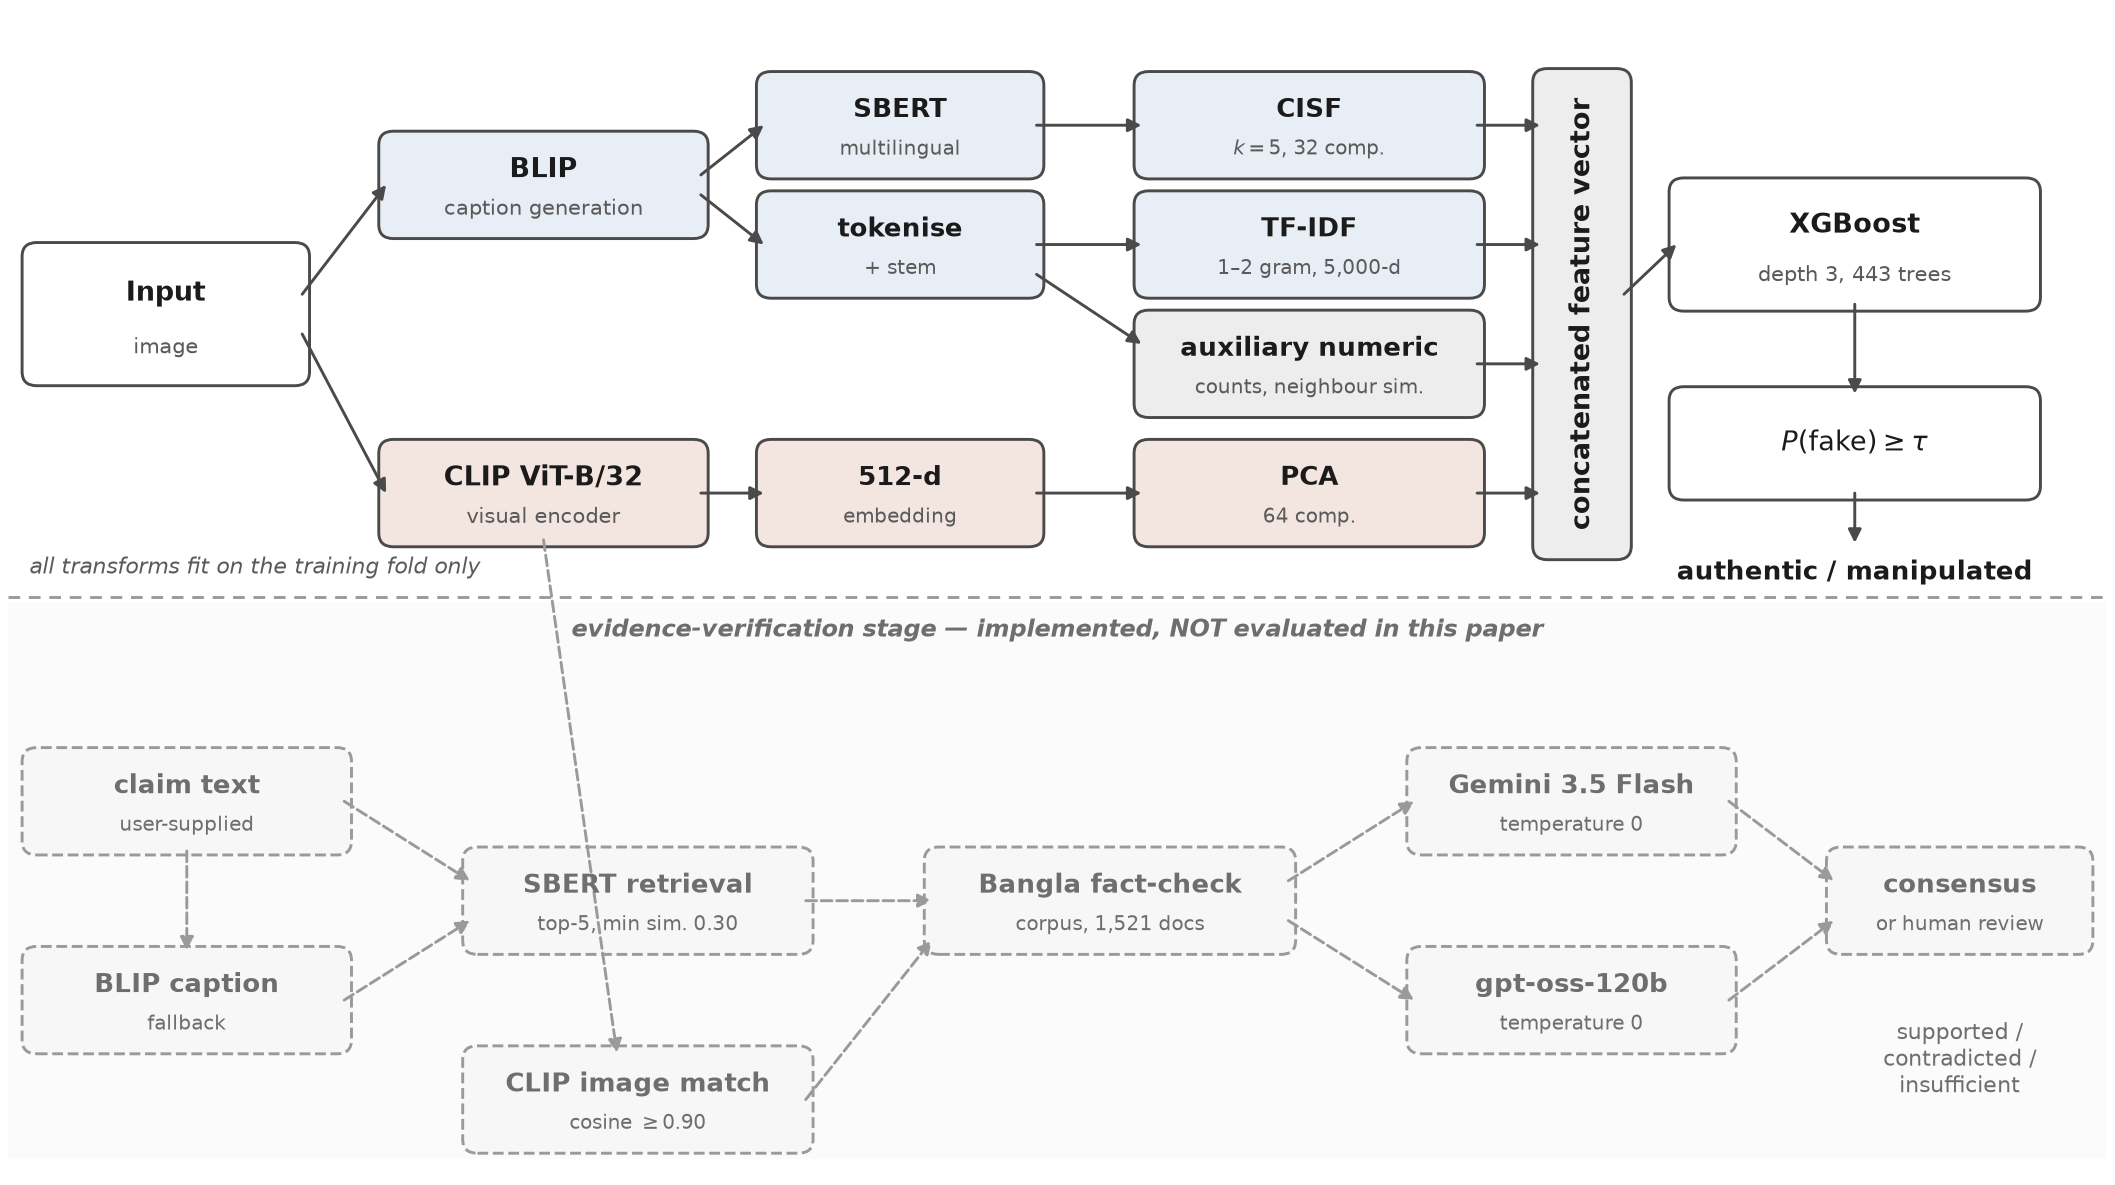
\includegraphics[width=0.80\textwidth]{fig1_system_architecture.png}
\caption{\sysname{} architecture. \textbf{Upper band (evaluated):} the four
feature blocks of Section~\ref{sec:features}, concatenated and classified by a
gradient-boosted tree; OCR is absent by design. \textbf{Lower band (dashed):}
the evidence-verification stage present in the implementation but not evaluated
here, and on which no result depends.}
\label{fig:arch}
\end{figure*}

\subsection{Dataset, Screening and Partitioning}
\label{sec:data}

The classifier is trained and evaluated on the AdversarialEdit split of the
public BanFakeMM benchmark \cite{banfakemm}, a detector-guided corpus built
from 7{,}040 authentic Bangla news articles across eleven topical categories:
2{,}000 images, 1{,}000 authentic and 1{,}000 manipulated. BanFakeMM
constructs its manipulated images through a defined editing or generation
pipeline rather than subjective annotation, so labels are deterministic by
construction.

Behaviour under distribution shift is measured on BanFakeMM's AdversarialGen
split, balanced in the same way---1{,}000 authentic images and 1{,}000 whose
manipulated counterpart is synthesised rather than edited---so the shift is in
how the \emph{positive} class is produced, not in the composition of the split.
Setting aside its distributed 80/10/10 partition, which does not suit a
three-way adaptation study, we repartition its 2{,}000 images at a fixed seed
(42): 300 for supervised adaptation, 150 for decision-threshold selection, and
200 sealed as the final test partition, used in no training, tuning or
threshold-selection step. The remaining 1{,}350 are unused.

\subsubsection{Near-duplicate screening}
\label{sec:dedup}
Filename comparison is not sufficient: a manipulated image is an edited copy
of an authentic one, so the two can carry unrelated names and still be the same
picture. All 2{,}650 images are screened by content, each reduced to a 64-bit
DCT perceptual hash (pHash), a 64-bit difference hash (dHash) and its CLIP
embedding; a pair is a near-duplicate when either Hamming distance is at most 2
or the CLIP cosine is at least 0.98, and pairs are merged with union-find.
These thresholds sit in a clear gap: of 3.5 million candidate pairs, 94 lie at
pHash distance 0 and only 102 at distance 6 or below. Duplicates are
near-exact, and looser settings chain unrelated images into implausible
clusters.

The screen links 118 pairs into 19 clusters covering 58 images. Ten span more
than one partition: 6 of the 200 sealed test images (3.0 percent), 2 of the 150
validation and 11 of the 300 adaptation images have a near-duplicate in the
base training set. These are removed from the two \emph{evaluation} partitions
and no replacements drawn, leaving a 194-image sealed test partition (100
manipulated, 94 authentic) and a 148-image validation partition---the
denominators used throughout.
The adaptation partition keeps all 300, of which 289 are novel relative to
base training: a duplicate inside training data is redundancy, not leakage, and
pruning it would confound the adaptation contrast with a change in training-set
size. What is verified is narrower than freedom from leakage: no evaluation
image shares a duplicate cluster with base training \emph{or} adaptation data. Within the base split
the screen yields 1{,}980 groups over 2{,}000 images, and every fold in
Section~\ref{sec:ablation} is built with \texttt{StratifiedGroupKFold} over
those groups, asserted group-disjoint at run time.

Provenance is published, and we use it to measure what the image screen cannot
catch. Every record carries an \texttt{article\_id}, and 1{,}863 ids in the
released master file carry both an authentic image and its manipulated
counterparts. Mapping all 2{,}650 study images to their records by content
hash, 40 evaluation images share an article with a training image while being
visually unrelated (median pHash distance 30 and CLIP cosine 0.52, against 32
and 0.40 for random pairs); only three are near-duplicates, and the image
screen had already removed those.

\emph{The remainder we keep, and limit the screening claim accordingly}: it
removes image duplicates, not shared-story information, which different pixels
do not rule out---a caption from the same event can carry it. Twenty such
images reach the sealed partition, all authentic; excluding them raises
accuracy by 0.7--1.1 points across every row of Table~\ref{tab:shift} and
leaves fake-recall unchanged, so article overlap inflates nothing---those
images are if anything slightly harder. That aggregates frozen predictions
rather than re-running under article-grouped training, and we claim only the
former.

\subsection{Features and Classifier}
\label{sec:features}

A BLIP model generates a caption per image; OCR was evaluated during ablation
and removed (Section~\ref{sec:ablation}). The caption is tokenized and stemmed,
with separate handling for Bangla and Latin script, for TF-IDF features, and
separately encoded by multilingual SBERT. That embedding is refined through
CISF: combined with the weighted average of its $k=5$ nearest training
neighbours at fusion weight $\alpha=0.65$, re-normalized, and reduced to 32
components. A CLIP vision encoder independently produces a
512-dimensional embedding, reduced to 64 components. These were fixed design
choices, not outcomes of a search; a sensitivity study, and comparison against
adaptive fusion \cite{mmfusionnet,claaf}, is left for future work.

The full vector concatenates four blocks, each fit only on the training fold:
the CISF caption embedding, the CLIP embedding, TF-IDF over the caption (1--2
grams, vocabulary capped at 5{,}000, minimum document frequency 3), and
auxiliary numeric features. Each training embedding's neighbour search excludes
itself, and at inference an unseen embedding is compared only against this
fixed training-set reference. Classification uses XGBoost
(\texttt{max\_depth}~3, \texttt{learning\_rate}~0.0742,
\texttt{n\_estimators}~443, \texttt{subsample}~0.866,
\texttt{colsample\_bytree}~0.683, \texttt{min\_child\_weight}~2,
\texttt{gamma}~0.143, \texttt{reg\_alpha}~$1.01\times10^{-5}$,
\texttt{reg\_lambda}~4.911), selected by randomized search over 8 sampled
configurations under 3-fold cross-validation.

\subsection{Threshold Selection and Metrics}
\label{sec:training}

The operating threshold is selected on held-out validation data, never on the
evaluation partition, under a rule fixed before the sweep was run: $\tau$
maximizes fake-class F1 on the screened 148-image validation partition over a
$0.01$-step grid, ties broken by the median of the tied run
(Fig.~\ref{fig:sweep}). The sealed 194-image test partition is then scored
exactly once at the resulting threshold, after all training and threshold
decisions are frozen, and is used for no tuning of any kind.

Ablation results come from repeated stratified 5-fold \emph{grouped}
cross-validation over the clusters of Section~\ref{sec:dedup} (2 repeats, 10
folds), with identical splits and fixed hyperparameters across every
configuration, and all transforms fit inside the training fold only. Every
same-distribution figure is computed at the conventional $\tau = 0.50$
cut-off: no threshold search is performed on the base split, so those numbers
carry no selection effect.

Results are reported as accuracy, precision, recall and F1 for the manipulated
class, with real-class recall added under shift. Fake-recall is the more
safety-critical metric---a missed manipulation circulates unchecked whereas a
false alarm costs only a review step---which is why the selection rule
maximizes fake-class F1.

Repeated cross-validation does not yield independent observations: each image
is held out once per repeat, and any two training folds overlap in four fifths
of their rows. We therefore never stack repeats. Out-of-fold probabilities are
averaged across repeats so each image contributes one prediction to any paired
test, and fold-level comparisons use the Nadeau--Bengio corrected resampled $t$
interval, which adds the train/test overlap ratio
($n_{\text{test}}/n_{\text{train}} = 0.25$ at five folds) to the naive $1/J$
variance term---a $3.5\times$ inflation here. The $\pm$ values in
Table~\ref{tab:ablation} are the spread across folds, not standard errors.
Bootstrap resampling is applied only to the sealed partition, scored once. Every random operation uses a fixed seed of 42;
manifests, per-image probabilities and the full validation sweep are released
with the code.

%==============================================================
\section{Experimental Results}
%==============================================================

\subsection{Per-Modality Ablation}
\label{sec:ablation}

\begin{table}[!tb]
\caption{Baselines and Per-Modality Ablation Under One Protocol: Repeated
Stratified 5-Fold \emph{Grouped} Cross-Validation Over Near-Duplicate Clusters
($2$ Repeats, $10$ Folds), in Percent.}
\label{tab:ablation}
\centering
\setlength{\tabcolsep}{3.5pt}
\footnotesize
\begin{tabular}{lcccc}
\toprule
\textbf{Configuration} & \textbf{Acc.} & \textbf{Prec.$_{f}$} &
\textbf{Rec.$_{f}$} & \textbf{F1$_{f}$} \\
\midrule
\multicolumn{5}{l}{\emph{Text-only baselines}} \\
Linear SVM (TF-IDF)     & 73.93 $\pm$ 1.35 & 72.42 & 77.40 & 74.80 \\
XGBoost (TF-IDF + num.) & 77.15 $\pm$ 1.86 & 77.50 & 76.60 & 77.00 \\
\midrule
\multicolumn{5}{l}{\emph{Modality ablation}} \\
OCR only              & 57.35 $\pm$ 2.34 & 63.97 & 33.85 & 44.22 \\
Caption only          & 74.50 $\pm$ 2.68 & 75.22 & 73.25 & 74.16 \\
Text only             & 76.05 $\pm$ 1.82 & 76.42 & 75.45 & 75.87 \\
Text + CISF           & 77.38 $\pm$ 2.10 & 77.41 & 77.55 & 77.40 \\
\midrule
CLIP only\,$^{\dagger}$ & 95.38 $\pm$ 1.33 & 94.68 & 96.15 & 95.41 \\
Text + CLIP           & 95.28 $\pm$ 1.04 & 95.04 & 95.55 & 95.28 \\
CLIP + CISF           & 95.23 $\pm$ 1.38 & 95.07 & 95.40 & 95.23 \\
Caption + CISF + CLIP & 95.40 $\pm$ 1.09 & 95.13 & 95.70 & 95.41 \\
\bottomrule
\multicolumn{5}{p{0.94\columnwidth}}{\footnotesize Subscript $f$ denotes the
manipulated class. No row is marked best: the four CLIP-containing
configurations are statistically indistinguishable (Section~\ref{sec:fusion}).
$^{\dagger}$ selected, on the calibration and cost grounds of
Section~\ref{sec:fusion}.}
\end{tabular}
\end{table}

\begin{figure}[!tb]
\centering
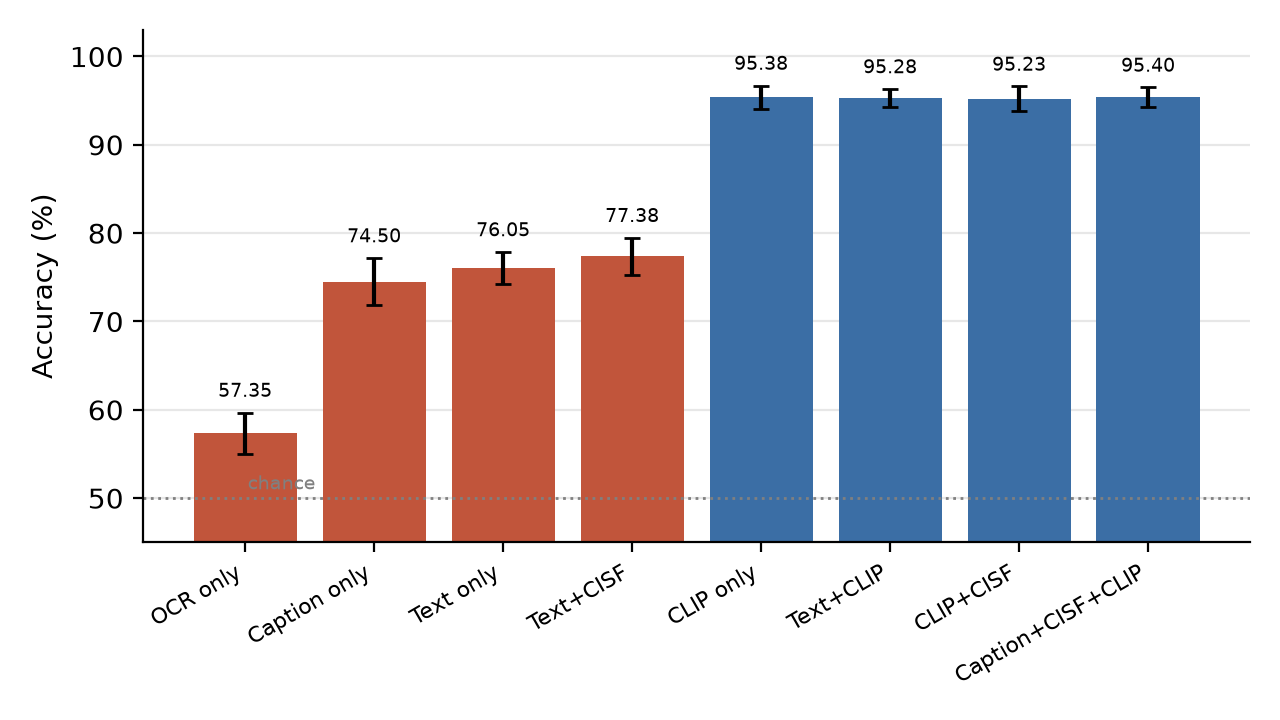
\includegraphics[width=0.95\columnwidth]{fig2_modality_ablation.png}
\caption{Per-modality ablation accuracy (repeated stratified 5-fold grouped
cross-validation; error bars are one standard deviation across folds).}
\label{fig:ablation}
\end{figure}

Table~\ref{tab:ablation} and Fig.~\ref{fig:ablation} report every configuration
under an identical protocol. OCR in isolation reaches 57.35 percent, near the
50 percent chance baseline, with fake-recall of only 33.85 percent; this is the
basis for removing it. All text-only configurations saturate below 78 percent
while any containing CLIP exceeds 95: BanFakeMM's manipulations are pixel-level
edits or full-image generations, so the evidence lies in visual texture and
generation artifacts, not in anything a caption records. The OCR result does
not generalize beyond this benchmark---MultiBanFakeDetect \cite{multibanfake}
indicates text-in-image remains a meaningful vector, and on such a corpus the
ranking could invert.

The third result is negative and we report it rather than obscure it: no
CLIP-containing configuration is distinguishable from any other, the spread
across the four being 0.17 points against a per-fold standard deviation of
1.0--1.4. The ranking even reverses under an unrelated methodological
change---ungrouped folds put CLIP-only ahead by 0.18 points, duplicate-aware
folds put the fused configuration ahead by 0.02---the clearest evidence it was
never resolvable. Section~\ref{sec:fusion} settles the choice on other
grounds.

\subsection{Does the Caption Pathway Contribute?}
\label{sec:fusion}

Accuracy parity does not settle whether the caption pathway is worth keeping:
a feature block can leave accuracy unchanged yet still improve ranking or
calibration, neither of which is visible in Table~\ref{tab:ablation}. We
therefore compare CLIP-only against the fused configuration on four measures in
both regimes, everything else held fixed.

\begin{table}[!tb]
\caption{CLIP-Only Versus the Fused Configuration, Same Hyperparameters and
Folds. AUROC and Brier Are Threshold-Independent; ECE Uses $10$ Bins. Arrows
Mark the Preferred Direction.}
\label{tab:fusion}
\centering
\setlength{\tabcolsep}{4pt}
\footnotesize
\begin{tabular}{llcccc}
\toprule
& \textbf{Model} & \textbf{Acc.}$\uparrow$ & \textbf{AUROC}$\uparrow$ &
\textbf{Brier}$\downarrow$ & \textbf{ECE}$\downarrow$ \\
\midrule
\multirow{2}{*}{\rotatebox{90}{\scriptsize same-d.}}
& CLIP only & 95.38 & 0.9918 & 0.0349 & 3.17 \\
& Fused     & 95.40 & 0.9920 & 0.0342 & 3.05 \\
\midrule
\multirow{2}{*}{\rotatebox{90}{\scriptsize shift}}
& CLIP only & 85.05 & \textbf{0.9759} & \textbf{0.0936} & \textbf{4.06} \\
& Fused     & 85.57 & 0.9732 & 0.1076 & 7.31 \\
\bottomrule
\multicolumn{6}{p{0.94\columnwidth}}{\footnotesize Same-distribution figures
are pooled out-of-fold values over the folds of Table~\ref{tab:ablation};
shift figures are the screened 194-image sealed partition at
$\tau = 0.50$, so both models are compared at the same operating point.}
\end{tabular}
\end{table}

Same-distribution, the two are indistinguishable on every measure. The paired
fold-level differences (fused minus CLIP-only), with the Nadeau--Bengio
correction for fold dependence, are $+0.03$ accuracy points (95\% CI
$[-0.98, +1.03]$, $p = 0.956$), $+0.0002$ AUROC ($p = 0.811$), $-0.0006$ Brier
($p = 0.709$) and $-0.12$ ECE points ($p = 0.794$); McNemar on the
repeat-averaged out-of-fold predictions, one per image, finds 21 images the
fused model alone classifies correctly against 20 for CLIP-only (exact
$p = 1.000$). Every interval spans zero, and the uncorrected intervals---which
we do not report---were $1.9\times$ narrower.

Under shift the comparison turns against the caption pathway. Its
$+0.5$-point accuracy advantage sits well inside its interval
($[-2.6, +3.6]$), while its calibration is clearly worse: Brier rises from
$0.0936$ to $0.1076$ and expected calibration error from $4.06$ to
$7.31$ points---least trustworthy exactly where the threshold has to be chosen.
The pathway costs a BLIP forward pass, an SBERT encoding and a
nearest-neighbour search per image and returns nothing measurable, so \emph{we
do not claim it as a contribution and adopt CLIP-only as the recommended
configuration}, evaluated in Section~\ref{sec:shift}.

\subsection{Performance Under Distribution Shift}
\label{sec:shift}

\begin{table}[!tb]
\caption{Evaluation Under Distribution Shift: the Recommended CLIP-Only Model
and the Fused Configuration Under an Identical Protocol. Thresholds Were
Selected on the Disjoint 148-Image Validation Partition; the Sealed 194-Image
Test Partition Was Scored Once Per Threshold. All Values in Percent.}
\label{tab:shift}
\centering
\setlength{\tabcolsep}{3pt}
\footnotesize
\begin{tabular}{llccccc}
\toprule
\textbf{Setting} & \textbf{$\tau$} & \textbf{Acc.} & \textbf{Prec.$_{f}$} &
\textbf{Rec.$_{f}$} & \textbf{Rec.$_{r}$} & \textbf{F1$_{f}$} \\
\midrule
\multicolumn{7}{l}{\emph{CLIP-only (recommended)}} \\
Zero-shot, default   & 0.50 & 85.1 & 94.9 & 75.0 & 95.7 & 83.8 \\
Zero-shot, val.-sel. & 0.09 & \textbf{91.2} & 88.1 & 96.0 & 86.2 & 91.9 \\
Adapted, val.-sel.   & 0.12 & 89.7 & 84.5 & 98.0 & 80.9 & 90.7 \\
\midrule
\multicolumn{7}{l}{\emph{Fused, caption + CISF + CLIP (for comparison)}} \\
Zero-shot, default   & 0.50 & 85.6 & 98.6 & 73.0 & 98.9 & 83.9 \\
Zero-shot, val.-sel. & 0.08 & \textbf{91.8} & 89.6 & 95.0 & 88.3 & 92.2 \\
Adapted, val.-sel.   & 0.21 & 91.8 & 90.4 & 94.0 & 89.4 & 92.2 \\
\bottomrule
\multicolumn{7}{p{0.95\columnwidth}}{\footnotesize Bootstrap 95\% CIs on
accuracy (5{,}000 resamples), validation-selected rows: CLIP-only
$[87.1, 94.8]$ and $[85.1, 93.8]$; fused $[87.6, 95.4]$ and $[87.6, 95.4]$.
Subscripts $f$ and $r$ denote the manipulated and authentic classes.}
\end{tabular}
\end{table}

\begin{figure}[!tb]
\centering
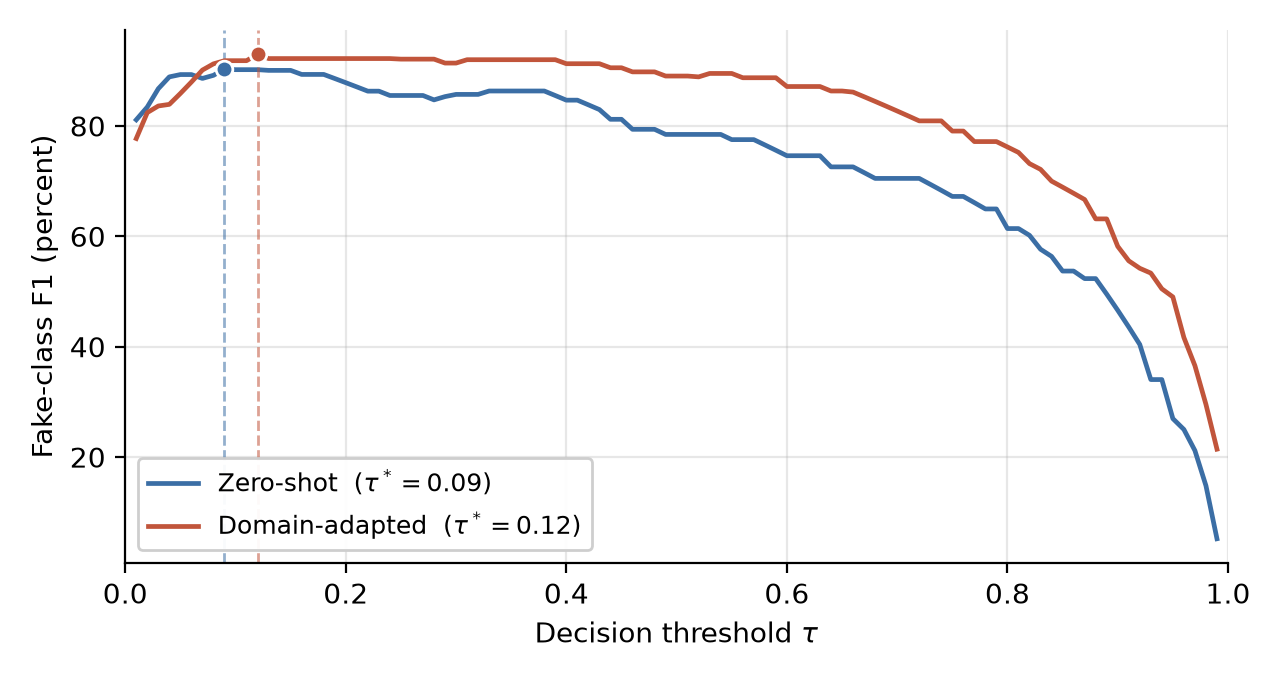
\includegraphics[width=0.95\columnwidth]{fig3_validation_threshold_sweep.png}
\caption{Fake-class F1 against decision threshold for the recommended
CLIP-only model on the 148-image validation partition: $\tau^{*} = 0.09$
zero-shot and $0.12$ domain-adapted, the values carried into
Table~\ref{tab:shift}. Both optima sit on a broad plateau. $\tau^{*}$ is the
argmax under the rule fixed in Section~\ref{sec:training}; the sealed test
partition plays no part in this selection.}
\label{fig:sweep}
\end{figure}

CLIP-only is the recommended configuration and the one evaluated here; the
fused model is carried through the identical protocol for comparison
(Table~\ref{tab:shift}). At the default threshold CLIP-only transfers poorly to the unseen manipulation
style: accuracy falls from 95.38 percent same-distribution to 85.1, and
fake-recall from 96.15 to 75.0. The 21.2-point fake-recall collapse, not the
10.3-point accuracy drop, is what matters operationally---25 of 100 manipulated
images pass undetected while only 4 of 94 authentic images are misflagged, an
asymmetry consistent with a boundary calibrated tightly around the training
distribution.

Applying the validation-selected threshold ($\tau = 0.09$), without retraining,
raises sealed-test accuracy to 91.2 percent (95 percent CI $[87.1, 94.8]$) and
fake-recall to 96.0, at a cost of 9.5 points of real-recall. Almost the entire
shift penalty is therefore calibration rather than failed visual
discrimination: the ranking already separates the classes, and only the
operating point was wrong. The fused model is nowhere distinguishable from it:
paired on the same 194 images, it leads by $+0.5$,
$+0.5$ and $+2.1$ points across the three settings of Table~\ref{tab:shift},
with 95 percent CIs of $[-2.6, +3.6]$, $[-2.1, +3.1]$ and $[-1.0, +5.7]$ and
McNemar $p \geq 0.39$. Its largest lead, on the adapted row, is also its least
certain---the same verdict Section~\ref{sec:fusion} reached by another
route.

\emph{Supervised adaptation adds nothing measurable, for either
configuration.} Retraining CLIP-only with 300 additional AdversarialGen images
and again selecting on validation ($\tau = 0.12$) gives 89.7 percent, $-1.5$
points against the zero-shot model (95 percent CI $[-4.6, +1.5]$, 4 versus 7
discordant); for the fused model the difference is $+0.0$ points (95 percent CI
$[-3.6, +3.6]$, McNemar $p = 1.00$ on 6 versus 6). Both intervals span
zero.

An earlier draft reported a 90.0 $\rightarrow$ 91.5 percent gain from this
step. We retract it, and do not claim to know why it disappeared: screening,
grouped folds, a correction to the CLIP feature extraction and the move of
threshold selection off the evaluation set all changed between drafts, and we
ran no controlled comparison that would attribute the change to any one of
them. We report the measurement under the present protocol---no gain, with an
interval spanning zero.

\begin{figure}[!tb]
\centering
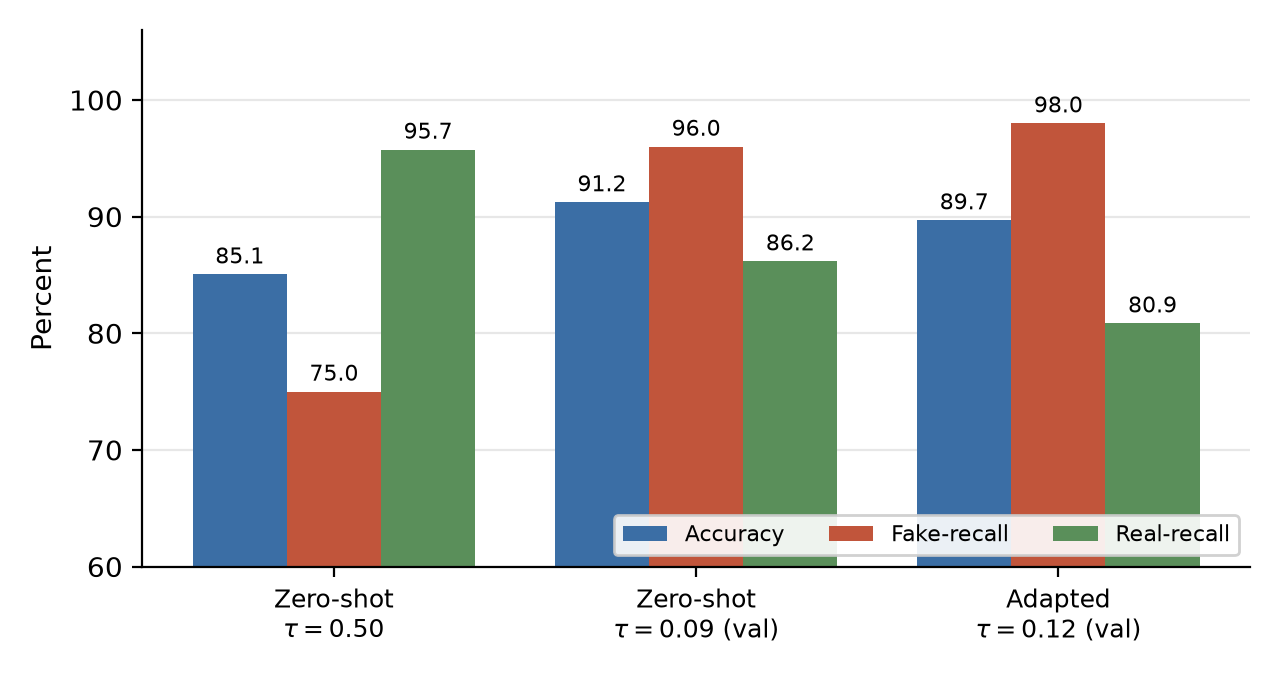
\includegraphics[width=0.95\columnwidth]{fig4_shift_performance.png}
\caption{Accuracy, fake-recall and real-recall for the recommended CLIP-only
model on the sealed test partition, across the three settings in the upper
block of Table~\ref{tab:shift}.}
\label{fig:progression}
\end{figure}

\begin{figure}[!tb]
\centering
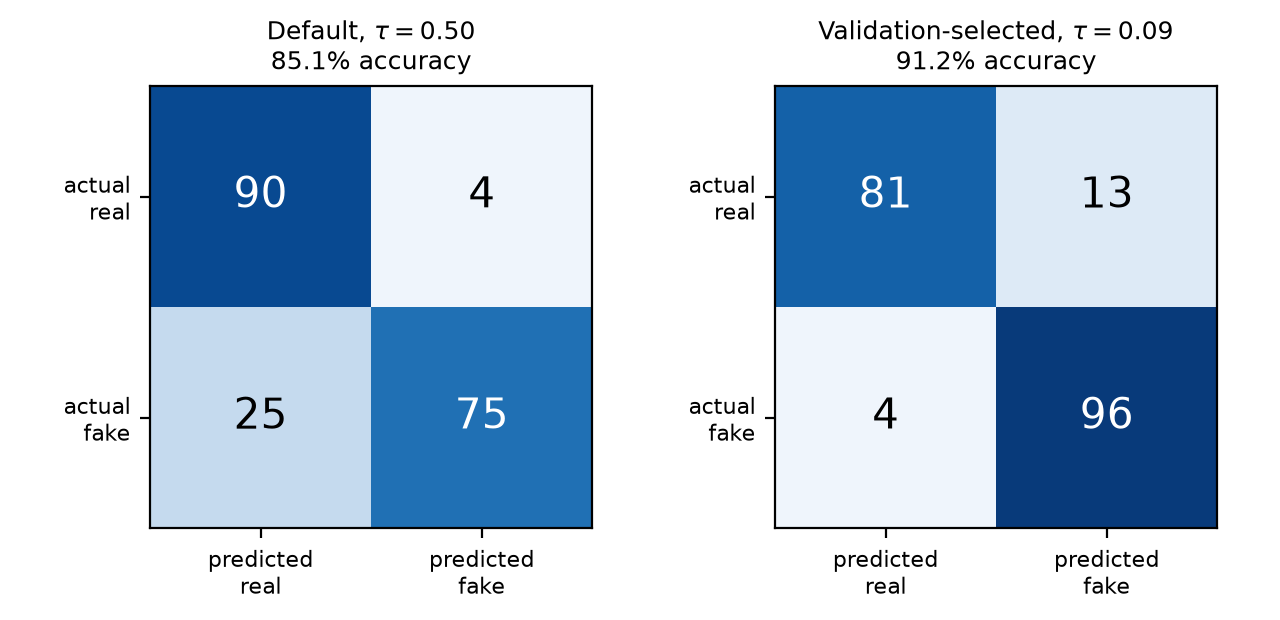
\includegraphics[width=0.95\columnwidth]{fig5_confusion_matrices.png}
\caption{Confusion matrices for the recommended CLIP-only model---the
\emph{same} zero-shot model at the default threshold (left) and at its
validation-selected threshold (right), so the contrast isolates calibration
from representation. The default cut-off misses 25 of 100 manipulated images;
the validation-selected one misses 4, at the cost of 9 further misflagged
authentic images.}
\label{fig:cm}
\end{figure}

Figs.~\ref{fig:progression} and~\ref{fig:cm} make the trade-off visible, and
the asymmetric cost argues for the validation-selected operating point. The
residual gap to the recommended model's 95.38 percent same-distribution
accuracy is an honest bound on demonstrated behaviour under shift.

\subsection{Baselines and the Cost of the Leak}

\begin{figure}[!tb]
\centering
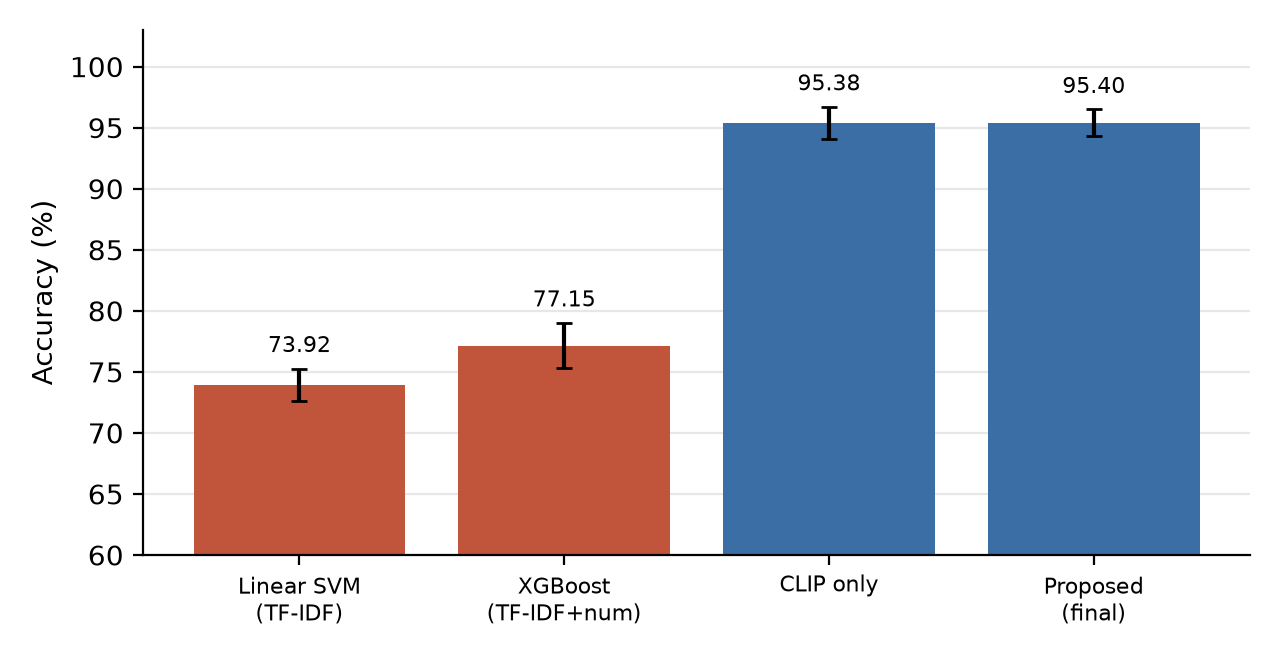
\includegraphics[width=0.95\columnwidth]{fig6_baseline_comparison.png}
\caption{CLIP-containing configurations against the text-only baselines under
the identical grouped cross-validation protocol.}
\label{fig:baselines}
\end{figure}

The two text-only baselines in Table~\ref{tab:ablation} sit 18--21 points below
any CLIP-containing configuration (Fig.~\ref{fig:baselines}), so the visual
branch is what separates this task. The comparison that decides the
system is not against these baselines but among the CLIP-containing rows, and
Section~\ref{sec:fusion} resolves it in favour of the simplest of them.

Which rows moved most when duplicate-aware folds replaced random ones is
itself informative: the text-only baselines lost 2.4 and 1.8 points while every
CLIP-containing configuration moved by at most 0.35. Near-duplicate images
share a BLIP caption almost verbatim, so a text model gains far more from the
leak---an argument for group-aware folds in caption-based work.

%==============================================================
\section{Discussion}
%==============================================================

\subsection{Calibration Versus Representation Under Shift}

The shift results separate two failure modes a single accuracy figure
conflates: a representation that does not transfer, and one that transfers
while its operating point does not. Ours is firmly the second---a threshold of
0.09, chosen without ever seeing the test partition, recovers 91.2 percent
accuracy and 96.0 percent fake-recall---so what failed at the default cut-off
was calibration, shifted manipulations receiving systematically lower
probabilities than training-style ones.

It also reframes what the 300 adaptation images were doing: under a
validation-selected threshold they add nothing, thresholding having already
captured the available headroom. Note the boundary: the two splits differ in how the
manipulated class is produced, not in image source, and a shift that also
changed provenance could plausibly damage the representation itself.

\subsection{Limitations and Future Directions}
\label{sec:limitations}

Ground-truth labels derive from BanFakeMM's deterministic construction, so the
demonstrated competence is specific to detecting algorithmic manipulation, not
to adjudicating a news item's claim: that a photograph was edited says nothing
about the story attached to it. The
distribution-shift evaluation, while sealed, screened and
free of threshold-selection effects, draws on a second split of the same
benchmark; generalization to sources outside BanFakeMM remains open. So does
article-level overlap: our folds and partitions are disjoint in image content
but not in source article, and we report its measured effect rather than
removing it.

Pairing this detector with retrieval over a Bangla fact-check corpus is the
obvious next step; evaluating one needs a labelled claim set with adjudicated
verdicts, retrieval recall@$k$ against gold evidence, and an abstention
analysis, so we do not report it. A preliminary measurement suggests it is
harder than it looks: the multilingual encoder we tested does not separate
Bangla fact-check headlines well enough, as they share a fixed rhetorical
template. Threshold calibration is also data-centric; alternatives such as
CLIPood \cite{clipood} and prompt tuning \cite{dpod} were not evaluated, and
video would need a different approach.

%==============================================================
\section{Conclusion}
%==============================================================

Practical Bangla misinformation detection demands more than a
same-distribution accuracy figure: it requires a distribution-shift check free
of selection effects and near-duplicate contamination, and an honest account of
what each component contributes.

This work contributes a classifier whose configuration was selected by
ablation rather than default inclusion---OCR removed after it proved near
chance, the caption pathway after it proved unjustified, leaving CLIP features
and a gradient-boosted tree; and a protocol whose safeguards are stated rather
than assumed---image-duplicate screening with residual article overlap
measured, disjoint adaptation, validation and sealed test subsets, a selection
rule fixed in advance, and a single scoring of the sealed
partition---quantifying a zero-shot gap (95.38 $\rightarrow$ 85.1 percent
accuracy, 96.15 $\rightarrow$ 75.0 percent fake-recall) that a
validation-selected threshold recovers to 91.2 percent without retraining.
Supervised adaptation adds nothing measurable once the threshold is chosen
honestly, for either configuration.

The gap between a high same-distribution figure and reliable behaviour outside
the training distribution is real---but our results locate most of it in
calibration rather than in the learned representation, which is both cheaper to
fix and easier to get wrong.

\ifblindsubmission\else
\section*{Acknowledgment}
The authors thank [NAMES] for their support of this work.
\fi

%==============================================================
\begin{thebibliography}{00}

\bibitem{banfakemm} A. F. C. Adiba, M. S. A. F. Alam, and M. S. Chowdhury,
``BanFakeMM: A multimodal Bangla fake news detection benchmark with progressive
adversarial attacks,'' Mendeley Data, V1, 2026, doi: 10.17632/3r9s7wfbh5.1.

\bibitem{banfakenews} M. Z. Hossain, M. A. Rahman, M. S. Islam, and S. Kar,
``BanFakeNews: A dataset for detecting fake news in Bangla,'' in
\emph{Proc. 12th Lang. Resources and Evaluation Conf. (LREC)}, 2020,
pp. 2862--2871.

\bibitem{multibanfake} F. T. J. Faria \emph{et al.}, ``MultiBanFakeDetect:
Integrating advanced fusion techniques for multimodal detection of Bangla fake
news in under-resourced contexts,'' \emph{Int. J. Inf. Manage. Data Insights},
2025.

\bibitem{banfakenews2} H. M. Shibu, S. Datta, M. S. Miah, N. Sami,
M. S. Chowdhury, and M. S. Islam, ``From scarcity to capability: Empowering
fake news detection in low-resource languages with LLMs,'' in
\emph{Proc. 1st Workshop Natural Lang. Process. Indo-Aryan and Dravidian Lang.
(IndoNLP)}, 2025, arXiv:2501.09604.

\bibitem{mmcfnd} S. Bansal, N. S. Singh, S. S. Dar, and N. Kumar, ``MMCFND:
Multimodal multilingual caption-aware fake news detection for low-resource
Indic languages,'' 2024, arXiv:2410.10407.

\bibitem{eann} Y. Wang \emph{et al.}, ``EANN: Event adversarial neural
networks for multi-modal fake news detection,'' in \emph{Proc. 24th ACM SIGKDD
Int. Conf. Knowl. Discovery Data Mining}, 2018, pp. 849--857.

\bibitem{mvae} D. Khattar, J. S. Goud, M. Gupta, and V. Varma, ``MVAE:
Multimodal variational autoencoder for fake news detection,'' in \emph{Proc.
World Wide Web Conf.}, 2019, pp. 2915--2921.

\bibitem{spotfake} S. Singhal, R. R. Shah, T. Chakraborty, P. Kumaraguru, and
S. Satoh, ``SpotFake: A multi-modal framework for fake news detection,'' in
\emph{Proc. IEEE 5th Int. Conf. Multimedia Big Data}, 2019, pp. 39--47.

\bibitem{defame} T. Braun, M. Rothermel, M. Rohrbach, and A. Rohrbach,
``DEFAME: Dynamic evidence-based fact-checking with multimodal experts,''
2024, arXiv:2412.10510.

\bibitem{ragar} M. A. Khaliq, P. Y.-C. Chang, M. Ma, B. Pflugfelder, and
F. Mileti\'{c}, ``RAGAR, your falsehood radar: RAG-augmented reasoning for
political fact-checking using multimodal large language models,'' in
\emph{Proc. 7th Fact Extraction and VERification Workshop (FEVER)}, ACL, 2024,
arXiv:2404.12065.

\bibitem{rama} S. Yang, Z. Yu, Z. Ying, Y. Dai, G. Wang, J. Lan, J. Xu,
J. Li, and E. C. H. Ngai, ``RAMA: Retrieval-augmented multi-agent framework for
misinformation detection in multimodal fact-checking,'' 2025,
arXiv:2507.09174.

\bibitem{calm} I.-H. Hsu \emph{et al.}, ``CaLM: Contrasting large and small
language models to verify grounded generation,'' in \emph{Findings ACL 2024},
arXiv:2406.05365.

\bibitem{mmfusionnet} J. He, T. Liu, J. Zhao, and B. Turner,
``MM-FusionNet: Context-aware dynamic fusion for multi-modal fake news
detection with large vision-language models,'' 2025, arXiv:2508.05684.

\bibitem{claaf} G. Mu, C. Chen, X. Li, Y. Chen, J. Dai, and J. Li, ``CLAAF:
Multimodal fake information detection based on contrastive learning and
adaptive agg-modality fusion,'' \emph{PLOS ONE}, May 2025.

\bibitem{clipood} Y. Shu, X. Guo, J. Wu, X. Wang, J. Wang, and M. Long,
``CLIPood: Generalizing CLIP to out-of-distributions,'' in \emph{Proc. 40th
Int. Conf. Machine Learning}, 2023, arXiv:2302.00864.

\bibitem{dpod} A. Bhattacharya, D. Brahma, S. N. Mahadev, A. Asati,
V. Verma, and S. Biswas, ``Can out-of-domain data help to learn domain-specific prompts for
multimodal misinformation detection?'' in \emph{Proc. IEEE/CVF WACV}, 2025,
arXiv:2311.16496.

\end{thebibliography}

%==============================================================
% IF STILL OVER 6 PAGES -- text first, so the figures survive:
%   1. Fig. 1 -> fig1_system_architecture_classifier_only.png (aspect 0.35
%      instead of 0.56). Same figure, half the height, saves ~0.20 page --
%      but it has no RAG band, so only do this if the limit forces it.
%   3. drop the FUSED block from Table III (4 rows); the fusion verdict then
%      rests on Table II alone. ~0.06 page. Do this LAST -- a reviewer asked
%      for CLIP-only and fusion to be evaluated side by side.
%   4. the second paragraph of Sec. IV-D (group-aware folds argument, ~60)
%   5. Table I rows "Caption only" and "Text only"
%
% DO NOT cut, whatever the page count: the dependence paragraph in Sec. III-D,
% the Nadeau-Bengio intervals in Sec. IV-B, the partitioning and provenance
% paragraphs in Sec. III-B, the retraction in Sec. IV-C. Each answers a
% specific reviewer point.
%
% IF UNDER 6 PAGES, restore in this order:
%   1. Fig. 1 back to 0.92\\textwidth and its longer caption
%   2. the tables back to full size (drop the \\footnotesize lines)
%   3. from iccit2026_full.tex: "Key Observations", then "Why Visual Features
%      Dominate", then "Addressing the Research Problems"
%==============================================================

\end{document}
